\subsection{Depth variation of isotope ratios --- basic visualization}
\setcounter{step}{0}

\goldbox{Writing done, images need to be updated}
During a~NanoSIMS measurement, the sample material is \bb{gradually eroded} by the primary ion beam while the emitted secondary ions are separated based on their mass and counted. The ion counts in the subsequent planes therefore record a~\bb{depth variation} of the elements and isotopes within the sample, making it possible to reconstruct their distribution in~3D. This section describes how to visualize this 3D variation in the most basic way: by displaying lateral profiles along depth in the sample.
\tcbe

In order to obtain a~good quality dataset for 3D reconstruction, the measurement needs to use a~relatively low primary ion current to achieve sufficient lateral resolution. At the same time, the same field of view on the sample needs to be measured repeatedly in \bb{many planes} to erode the sample along a~substantial depth interval (several microns) such that a~meaningful 3D variation in this interval occurs. The number of detected planes can start from several hundreds but can reach up to several thousands of planes (the example below will use 2500 planes). However, one NanoSIMS measurement in the imaging mode is limited to a~maximum of 1000 planes. This means that several measurements of the same sample area need to be done in sequence, leading to multiple raw data files that should be merged and analyzed as one file. Thus, the challenge of isotope ratio visualization along depth additionally includes a~need to load multiple raw files and merge them into a~single stack with potentially several thousands of images. 

Last but not least, it is useful to note that because ion count rates for minor isotopes (e.g., ${}^{13}C$) are typically very low, ion count ratios derived from those minor isotopes (e.g., \ttt{13C/12C}) will generally be noisy if based on data in a~single plane. To maximize the signal-to-noise ratio in depth profiles of isotope ratios while maintaining an acceptable depth resolution, it is better to handle the original ion count data in \bb{blocks} of multiple subsequent planes, where the counts in each block are summed up (across the planes but separately for each pixel in the lateral dimension) and treated as \bb{one} plane.  

Overall, basic visualization of the 3D variation in isotope ratios involves three major steps: (i) loading the raw data in blocks, possibly involving merging of multiple raw datasets, (ii) drift-correcting the planes within each block before they are summed up into a~single plane, and finally (iii) visualization of lateral profiles along depth. This section describes how to do these processing steps in LANS. The example uses datasets \ttt{xxx}, which are available in the same location as the Look@NanoSIMS program. They correspond to 3~consecutive scans of cable bacteria placed on a~polycarbonate filter, each comprizing 1000 planes.

\subsubsection{Loading datasets in blocks, merging multiple datasets}
\setcounter{step}{0}

\s In preparation for the subsequent steps, first select \lans{Input} $\ra$ \lans{Load raw dataset} to load \bb{all} planes in the first dataset.

\bul This step is required to determine the \lanstf{base mass for alignment} and \lanstf{special region for alignment}, which are required later on for drift-correcting planes in a~block.

\s Proceed as described in Sections \ref{sec:display-masses-plane-by-plane} (steps 1--3) and \ref{sec:drift-correction-accumulation} (steps 1--2) to define the \lanstf{base mass for alignment} and \lanstf{special region for alignment}.

\bul At this stage, you should \emph{not} proceed with image accumulation (steps 3--4 in Section~\ref{sec:drift-correction-accumulation}) just yet, because the planes need to be first drift-corrected and accumulated \emph{within} blocks.

\s Select \lans{Input} $\ra$ \lans{Load multiple RAW datasets in blocks}. 

\bul Navigate to the raw files and select them, using the \ttt{Ctrl} key to select multiple files.

\bul Note that this function does \emph{not} require you to load multiple datasets. You can also load planes in blocks for just one dataset. If you do load multiple datasets, however, make sure that they have been acquired with the same pixel resolution (e.g., $256\times 256$ pixels).

\s In the dialog window that opens, specify the \lanstf{block size}, i.e., the number of planes per block. If you are going to load data from multiple datasets, indicate whether or not you want to be able to specify a~different block size for each individual dataset.

\bul In this example, you will use the block size of 40 for the first two datasets and 20 for the third dataset. This is because the last dataset was (accidentally) acquired with $2\times$ longer dwell time than the first two datasets. Thus, in the dialog window, enter 40 for the block size and 1 (\ttt{=yes}) in the second field.

\s Click OK in the dialog window and observe the progress of loading in the Matlab console.

\bul First, the raw data will be loaded. Then, the drift-correction information for planes in each block will be calculated based on the values for \lanstf{Base mass for alignment} and \lanstf{Special region for alignment} (see Step~2 above). Subsequently, this information will be applied to drift-correct and accumulate planes in blocks for each mass.

\bul If you selected multiple raw datasets, the same steps will be repeated for each of them.

\bul After this step is completed, the dataset loaded in LANS will ``behave'' as any other raw dataset loaded via \lans{Input} $\ra$ \lans{Load RAW dataset}. The only difference will be that the individual planes are, in fact, a~sum of multiple planes. Thus, the subsequent analysis will proceed according to the same steps as for any other dataset. 

\s In particular, you need to start with the drift-correction and accumulation of planes via \lans{Input} $\ra$ \lans{Accumulate plane images} (Section~\ref{sec:drift-correction-accumulation}, steps 3--4). 

\bul This is because although the individual planes were drift-corrected \emph{within} each block (during the loading process), the drift-correction also needs to be calculated and applied \emph{between} blocks.

\s Select \lans{Output} $\ra$ \lans{Save FULL PROCESSED data} to save the image stack, for all masses and all planes, in a~Matlab format (extension \ttt{mat}).

\bul This is highly recommended because the loading of data in blocks, accompanied with drift-correction and accumulation, is quite laborious and may be time consuming. Thus, you likely do not want to do it again for the very same dataset or group of datasets. 

\bul When saving the data, use the default filename suggested by LANS, unless you really want to use a~different one. Note that the default filename will end with \ttt{bN.mat}, where \ttt{b} refers to the fact that it corresponds to data loaded in blocks and \ttt{N} corresponds to the number of planes per block (block size).

\bul Beware that if the final dataset contains many planes, the exported \ttt{mat} file can be quite large (e.g., hundreds of Mb). Still, this is an acceptable price to pay for not having to load the same multiple datasets in blocks again.

%%

\subsubsection{Visualization of lateral profiles along depth in the sample}
\setcounter{step}{0}

Although you can perform this analysis with any NanoSIMS dataset, it is most useful for datasets that have been loaded in blocks, as described in the previous section.

\s In the main LANS window, select the \lanscb{Display lateral profiles} checkbox in the \ttt{Output options} box. 

\bul If you only want to focus on lateral profiles, it is a~good idea if you deselect all other checkboxes (except those for exporting ASCII data and PDF graphics).

\s In the \lanstf{expression} and \lanstf{scale} fields, specify the formulas for the ion count ratios you want to analyze and the corresponding scale. 

\bul In this example, you will look at depth profiles of ${}^{13}C/^{12}C$, ${}^{18}O/^{16}O$, CN, P and O. Thus, enter \ttt{13C14N/12C14N}, \ttt{18O/16O}, \ttt{12C14N}, \ttt{31P} and \ttt{16O} in the expression fields. Then experiment with the optimal scales.

\bul Do not forget to check the corresponding checkboxes next to the formulas.

\s Select \lans{Output} $\ra$ \lans{Display ratios}. 

\s In the top-left corner of the new window that opens (Fig.~\ref{fig:lateral}A), select the variable based on which you want to define a~lateral profile.

\begin{figure}[!ht]
\centering
\begin{tabular}{cc}
A: 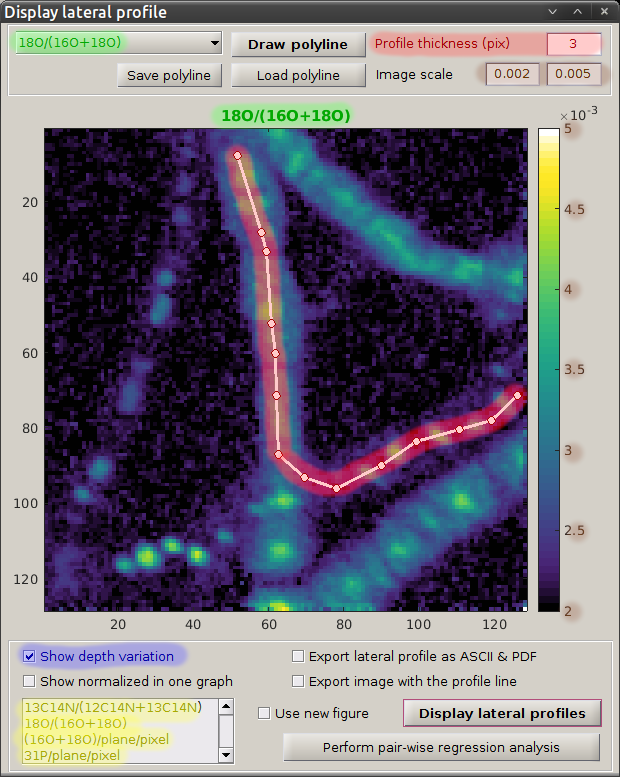
\includegraphics[scale=0.33, valign=t]{figs3/LANS-lateral1}
&
B: 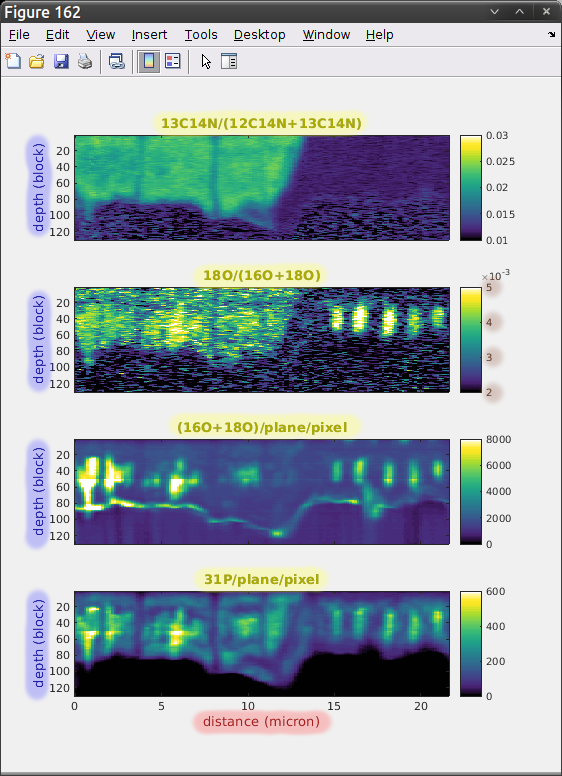
\includegraphics[scale=0.33, valign=t]{figs3/LANS-lateral2}
\end{tabular}
\caption{\label{fig:lateral}%
(A) LANS window for the analysis of variation in ion counts and ion count ratios along a~lateral profile. If the \lanscb{Show depth variation} checkbox is selected (marked in blue), the variation along depth will be displayed as well. (B) Results of this particular analysis show, among other things, that polyphosphate inclusions, visible as round areas (in both lateral and depth directions) with markedly higher signals of $P$ and $O$, are roughly homeogeneusly enriched in ${}^{18}O$ relative to the rest of the cell biomass.}
\end{figure}

\bul In this example, you will look at depth variation in the ${}^{18}O/^{16}O$ ratio in polyphosphate inclusions. Thus, select \ttt{18O/16O}.

\s Click on \lans{Draw polyline} to draw a~lateral profile in the image.

\bul The profile can have multiple vertices (hence the name `polyline'), allowing you to create profiles along a~``curved'' profile or even make sharp corners (Fig.~\ref{fig:lateral}A).

\bul Double-click to define the last vertex on the polyline. Although this will stop the polyline drawing mode, you can still continue adding, moving or removing vertices after this point by clicking with the right mouse button on the polyline. You can also move the entire polyline or remove it and start over.

\s Specify the \lanstf{Profile thickness}, in pixels.

\bul For the default value of 1, the lateral profile will be based on values in one pixel nearest to the polyline. Because this may yield a~rather noisy output, it is recommended to use a~greater value here. For example, using a~value of 5~for the profile thickness, the lateral profile will be based on values in 5~pixels nearest to the polyline (2~on one side, 2~on the other side, 1~on the polyline). Thus, you can think of the profile as being based on data in a~`band' following the polyline.

\s Select the \lanscb{Show depth variation} checkbox (highlighted in blue in Fig.~\ref{fig:lateral}A).

\s In the list of variables (highlighted in yellow in Fig.~\ref{fig:lateral}A), select variables that you want to analyze simultaneously.

\bul Hold \ttt{Ctrl} to select multiple variables. In this example, select all variables.

\s Click on \lans{Display lateral profiles}.

\bul This will open a new window showing the variation of the selected variables along the lateral profile (`band') and depth (Fig.~\ref{fig:lateral}B).

\s Select the \lanscb{Export} checkboxes to export the results as ASCII text and PDF images.

\s Click on \lans{Save polyline} to save the polyline coordinates.

\bul You can load it in the future by clicking on \lans{Load polyline}.
